\section*{Homework 4: AMPL Book Exercise 1-2}

\textbf{Problem:} The steel model for this chapter can be further modified to reflect various changes in production requirements. For each part below, explain the modifications to Figures 1-6a and 1-6b that would be required to achieve the desired changes. Make each change in isolation, not carrying modifications from part to part. 

\subsection*{Reference Information}

Before we begin, let's just keep the default info and solution up here as an easy reference. 

\noindent\textbf{Files:} Figures 1-6a and 1-6b both use the \textbf{steel4} .dat and .mod files. So I'll be using them as a base and modifying them. 

\noindent\textbf{steel4.mod}

\begin{lstlisting}
set PROD;   # products
set STAGE;  # stages

param rate {PROD,STAGE} > 0; # tons per hour in each stage
param avail {STAGE} >= 0;    # hours available/week in each stage
param profit {PROD};         # profit per ton

param commit {PROD} >= 0;    # lower limit on tons sold in week
param market {PROD} >= 0;    # upper limit on tons sold in week

var Make {p in PROD} >= commit[p], <= market[p]; # tons produced

maximize Total_Profit: sum {p in PROD} profit[p] * Make[p];

               # Objective: total profits from all products

subject to Time {s in STAGE}:
   sum {p in PROD} (1/rate[p,s]) * Make[p] <= avail[s];

               # In each stage: total of hours used by all
               # products may not exceed hours available

\end{lstlisting}

\noindent\textbf{steel4.dat}

\begin{lstlisting}
data;

set PROD := bands coils plate;
set STAGE := reheat roll;

param rate:  reheat  roll :=
  bands        200    200
  coils        200    140
  plate        200    160 ;

param:    profit  commit  market :=
  bands     25     1000    6000
  coils     30      500    4000
  plate     29      750    3500 ;

param avail :=  reheat 35   roll   40 ;
\end{lstlisting}


This provides the following solution:

\begin{align*}
	\text{Total Profit} &\approx 190071.43 \\
	\text{Bands} &\approx 3357.14 \\
	\text{Coils} &= 500 \\
	\text{Plates} &\approx 3142.86 \\
\end{align*}

As for time used, we use 35 hours on the reheat stage and 40 hours on the roll stage.

\subsection*{A \checkmark Checked on September 11.}

\textbf{Problem:} How would you change the constraints so that total hours used by all products must equal the total hours available for each stage? Solve the linear program and verify that you get the same results. Why is there no difference in solution?

\noindent\textbf{Solution:} All we need to do here is modify one line. Line 18 specifically. We change the $\leq$ to a strict $=$. 

\begin{lstlisting}
subject to Time: sum {p in PROD} (1/rate[p,s]) * Make[p] = avail[s];
\end{lstlisting}

The solution it gives is the exact same. This is because our goal is to produce as much as we can to maximize profit. So the original solution is already using up all of the available hours. We can check this programmatically and check the hours both solutions used. I don't have that included in here, but I personally verified that this was the case. 

\subsection*{B}

\textbf{Problem:} How would you add to the model to restrict the total weight of all products to be less than a new parameter, max\_weight? Solve the linear program for a weight limit of 6500 tons, and explain how this extract restriction changes the results.

\noindent\textbf{Solution:} We need to make a few modifications here. We'll need to edit both the .dat and .mod files. In the data file we simply add a new \texttt{max\_weight} parameter. Here it is next to \texttt{avail} for reference. Note that this parameter does not set specific weight limits for each product. 

\begin{lstlisting}
param avail := reheat 35 roll 40;
param max_weight := 6500; 
\end{lstlisting}

In the model file we read in this parameter and set a constraint for it. Firstly, we want the max weight to be a non-negative value. This is just a data quality check. 

After that, we create a new constraint using this parameter. This constraint ensures that the total weight across all products does not exceed \texttt{max\_weight}. 

\begin{lstlisting}
param max_weight >= 0		# Total tons of weight allowed across all products

subject to Total_Weight:
	sum{p in PROD} Make[p] <= max_weight;
\end{lstlisting}

Below is the solution generated after these modifications. 

\begin{align*}
	\text{Total Profit} &\approx 183791.67 \\
	\text{Bands} &\approx 1541.67 \\
	\text{Coils} &\approx 1458.33 \\
	\text{Plates} &= 3500 \\
\end{align*}

What we see is a substantial shift from the original solution. Production of bands is nearly halved and production of coils is nearly tripled. The production of plates reaches its maximum. Total profit compared to the original solution drops by around $\$6000$.

This is caused by the new constraint on total weight. In the original problem, production was only limited by the products rates in each stage and their availability. Though there were hard minimum and maximums on production for each product, this was never directly involved in the objective function. As such, profit per ton played no real part in the optimization process and \texttt{rate} was the main parameter dictating which products were prioritized.

The new total weight constraint forces the model to consider the profit per ton of each product. Coils are the slowest to produce, but they have the highest profit per ton value (30) followed by plates (29). Bands, meanwhile, have the lowest profit per ton (25) and are produced far less as a result. This solution maxes out plates because they are just barely the second most profitable per ton and are the second fastest to produce. Then bands and coils fill in the remaining allocation. This is also why the total profit is lower now as production can't just focus production on the heaviest products. 

\subsection*{C \checkmark Checked on September 11.}

\textbf{Problem:} How would you change the objective function to maximize total tons? Does this make a difference to the solution?

\noindent\textbf{Solution:} This is the simplest to change. Just remove the profit from the objective function as it already factors in weight. 

\begin{lstlisting}
	maximize Total_Weight: sum {p in PROD} Make[p];
\end{lstlisting}

Funnily enough this ends up with the exact same results as the original model!

\begin{align*}
	\text{Total Weight} &= 7000 \\
	\text{Bands} &\approx 3357.14 \\
	\text{Coils} &= 500 \\
	\text{Plates} &\approx 3142.86 \\
\end{align*}

We just don't get our profit shown in the objective function is all as it shows the total weight. The profit is the exact same as well, it just isn't shown here.

\subsection*{D}

\textbf{Problem:} Suppose that instead of the lower bounds represented by \texttt{commit[p]} in our model, we want to require that each product represent a certain share of the total tons produced. In the algebraic notation of Figure 1-1, this new constraint might be represented as

\[
	X_j \geq s_j \sum_{k \in P} X_k, \; \text{for each} \; j \in P
\]

where $s_j$ is the minimum share associated with project $j$. How would you change the AMPL model to use this constraint in place of the lower bounds \texttt{commit[p]}? If the minimum shares are 0.4 for bands and plate, and 0.1 for coils, what is the solution?

Verify that if you change the minimum shares to 0.5 for bands and plate, and 0.1 for coils, the linear program gives an optimal solution that produces nothing, at zero profit. Explain why this makes sense.

\noindent\textbf{Solution:} To start, we update the data file to remove the \texttt{commit} parameter and replace it with the new \texttt{share} parameter. 

\begin{lstlisting}
	param:    profit  market  share :=
	  bands     25    6000   0.4
	  coils     30    4000   0.1
	  plate     29    3500   0.4 ;
\end{lstlisting}

Next, in the model file, we remove the lower bound on \texttt{Make} set by \texttt{commit} and add a new constraint enforcing the minimum \texttt{share}.

\begin{lstlisting}
	param share {PROD} >= 0;     # minimum proportion of total tons for each product

	var Make {p in PROD} >= 0, <= market[p]; # tons produced

	subject to Share {p in PROD}:
	    Make[p] >= share[p] * sum {k in PROD} Make[k];
\end{lstlisting}

With this our new solution is as follows:

\begin{align*}
	\text{Total Profit} &= 189700 \\
	\text{Bands} &= 3500 \\
	\text{Coils} &= 700 \\
	\text{Plates} &= 2800 \\
\end{align*}

Firstly, this solution meets all minimum share requirements. The number of coils produced compared to the original solution increases by $200$ as a result of this change. 

Modifying the data file to shares of 0.5, 0.1, 0.5 results in no feasible solutions existing. As such, the optimizer produces nothing. This is because the shares are a proportion of the total production and the sum of these cannot exceed $1$ which this group of shares does. 

This shows some important behavior in AMPL. If the data and constraints provided result in no feasible solution then there will be no production. There has to be a feasible region for the solver to work with. 

\subsection*{E}

\textbf{Problem:} Suppose there is an additional finishing stage for plates only, with a capacity for 20 hours and a rate of 150 ton per hour. Explain how you could modify this data, without changing the model, to incorporate this new stage. 

\noindent\textbf{Solution:} This is actually, thankfully, very easy to do! We can simply add a new stage to the data file and set arbitrarily large limits for bands and coils.

\begin{lstlisting}
	set STAGE := reheat roll finishing;

	param rate:  reheat  roll  finishing:=
	  bands        200    200  infinity
	  coils        200    140  infinity
	  plate        200    160  150;

	param avail := reheat 35 roll 40 finishing 20;
\end{lstlisting}

This automatically gets worked in with 0 modifications to the model file! Below shows the run in Python.

\begin{figure}[htbp]
    \centering
    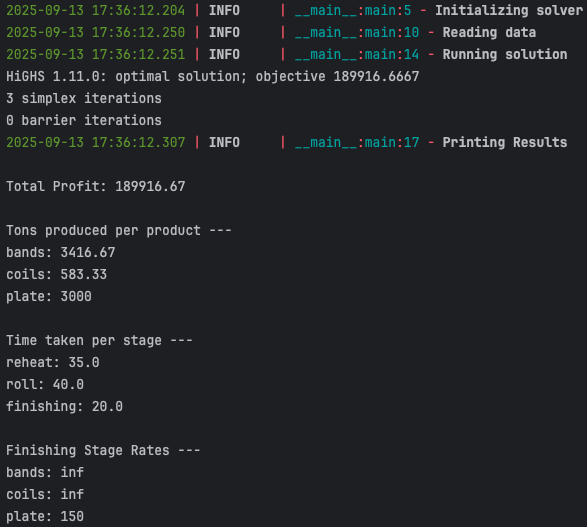
\includegraphics[width=0.8\textwidth]{../images/hw4-part-e-run.png}
    \caption{AMPL code running with finishing stage included.}
    \label{fig:your_label}
\end{figure}